

\tikzset{every picture/.style={line width=0.75pt}} %set default line width to 0.75pt        

\begin{tikzpicture}[x=0.75pt,y=0.75pt,yscale=-1,xscale=1]
%uncomment if require: \path (0,300); %set diagram left start at 0, and has height of 300

%Shape: Rectangle [id:dp05948589068926391] 
\draw  [color={rgb, 255:red, 144; green, 19; blue, 254 }  ,draw opacity=1 ][fill={rgb, 255:red, 255; green, 255; blue, 255 }  ,fill opacity=1 ][line width=2.25] [blur shadow={shadow xshift=0pt,shadow yshift=0pt, shadow blur radius=1.5pt, shadow blur steps=4 ,shadow opacity=100}] (23,74.5) -- (160,74.5) -- (160,218) -- (23,218) -- cycle ;
%Image [id:dp5741033059414491] 
\draw (279.44,145.67) node  {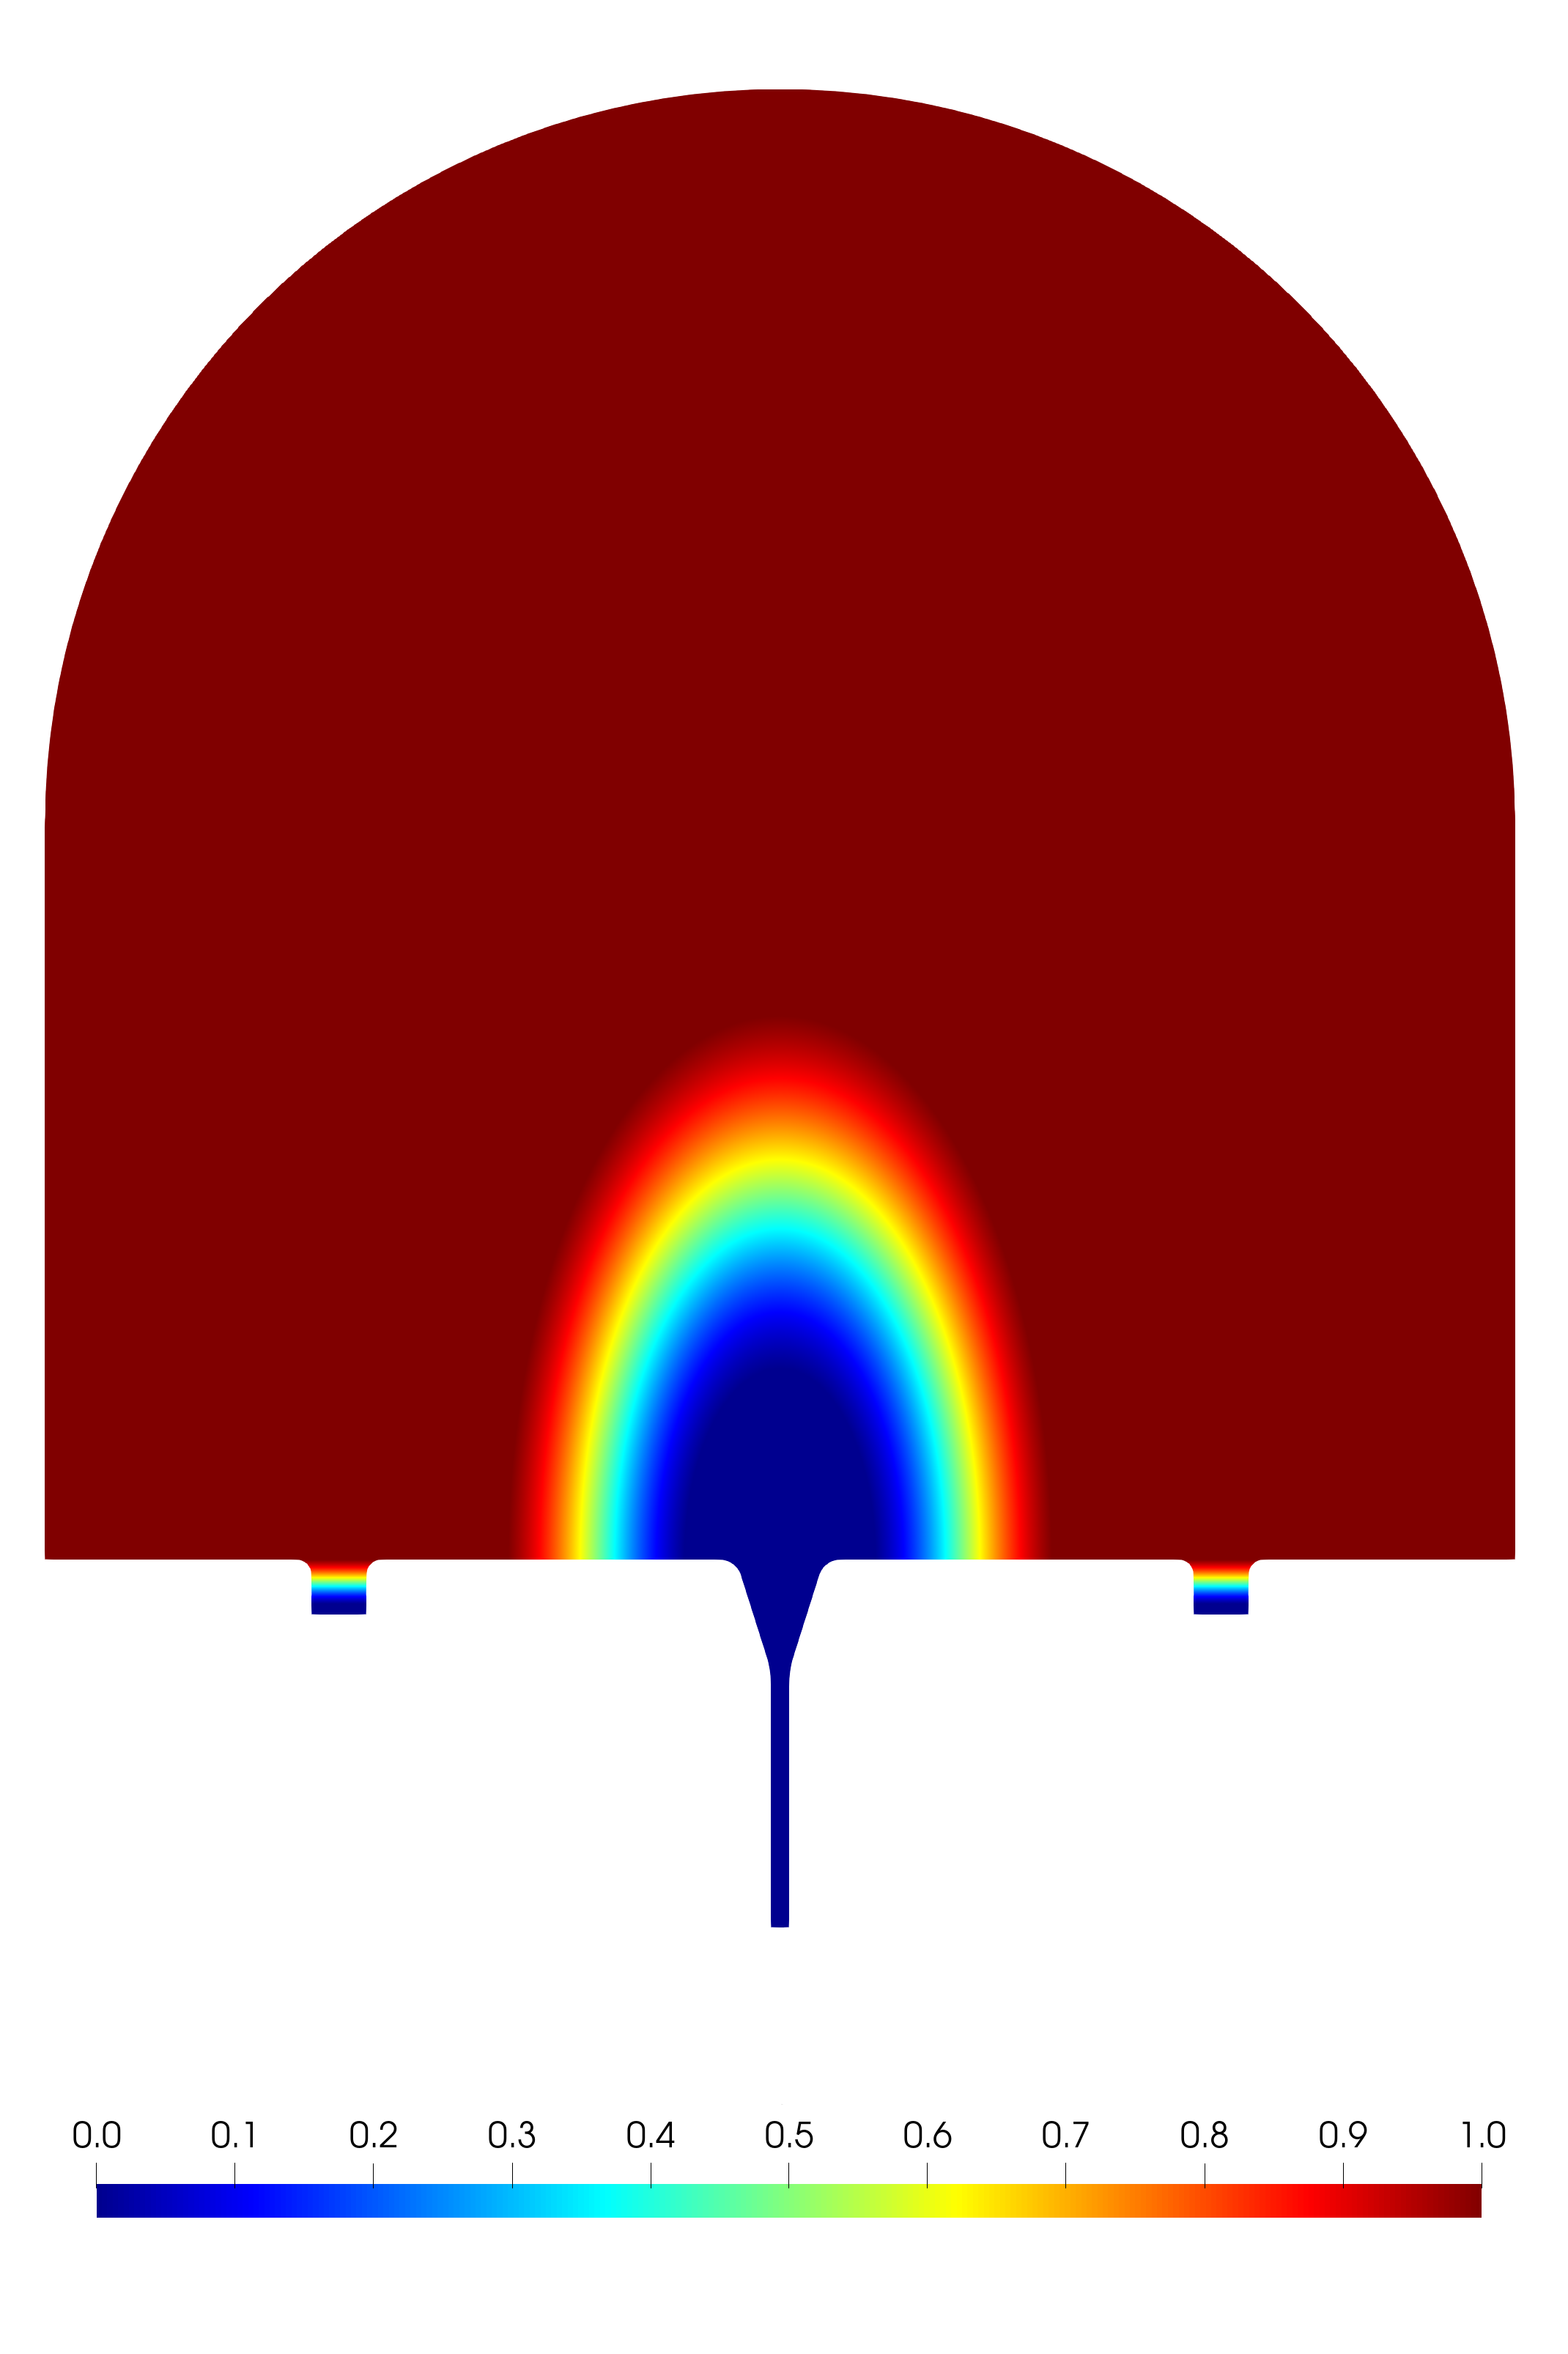
\includegraphics[width=142.91pt,height=214.5pt]{diagrams/results-modelling/velocity-transport/meshandsoln_cg_permeability_placenta_nsb_permeability-linear.png}};
%Image [id:dp5031667319380262] 
\draw (90.5,171.72) node  {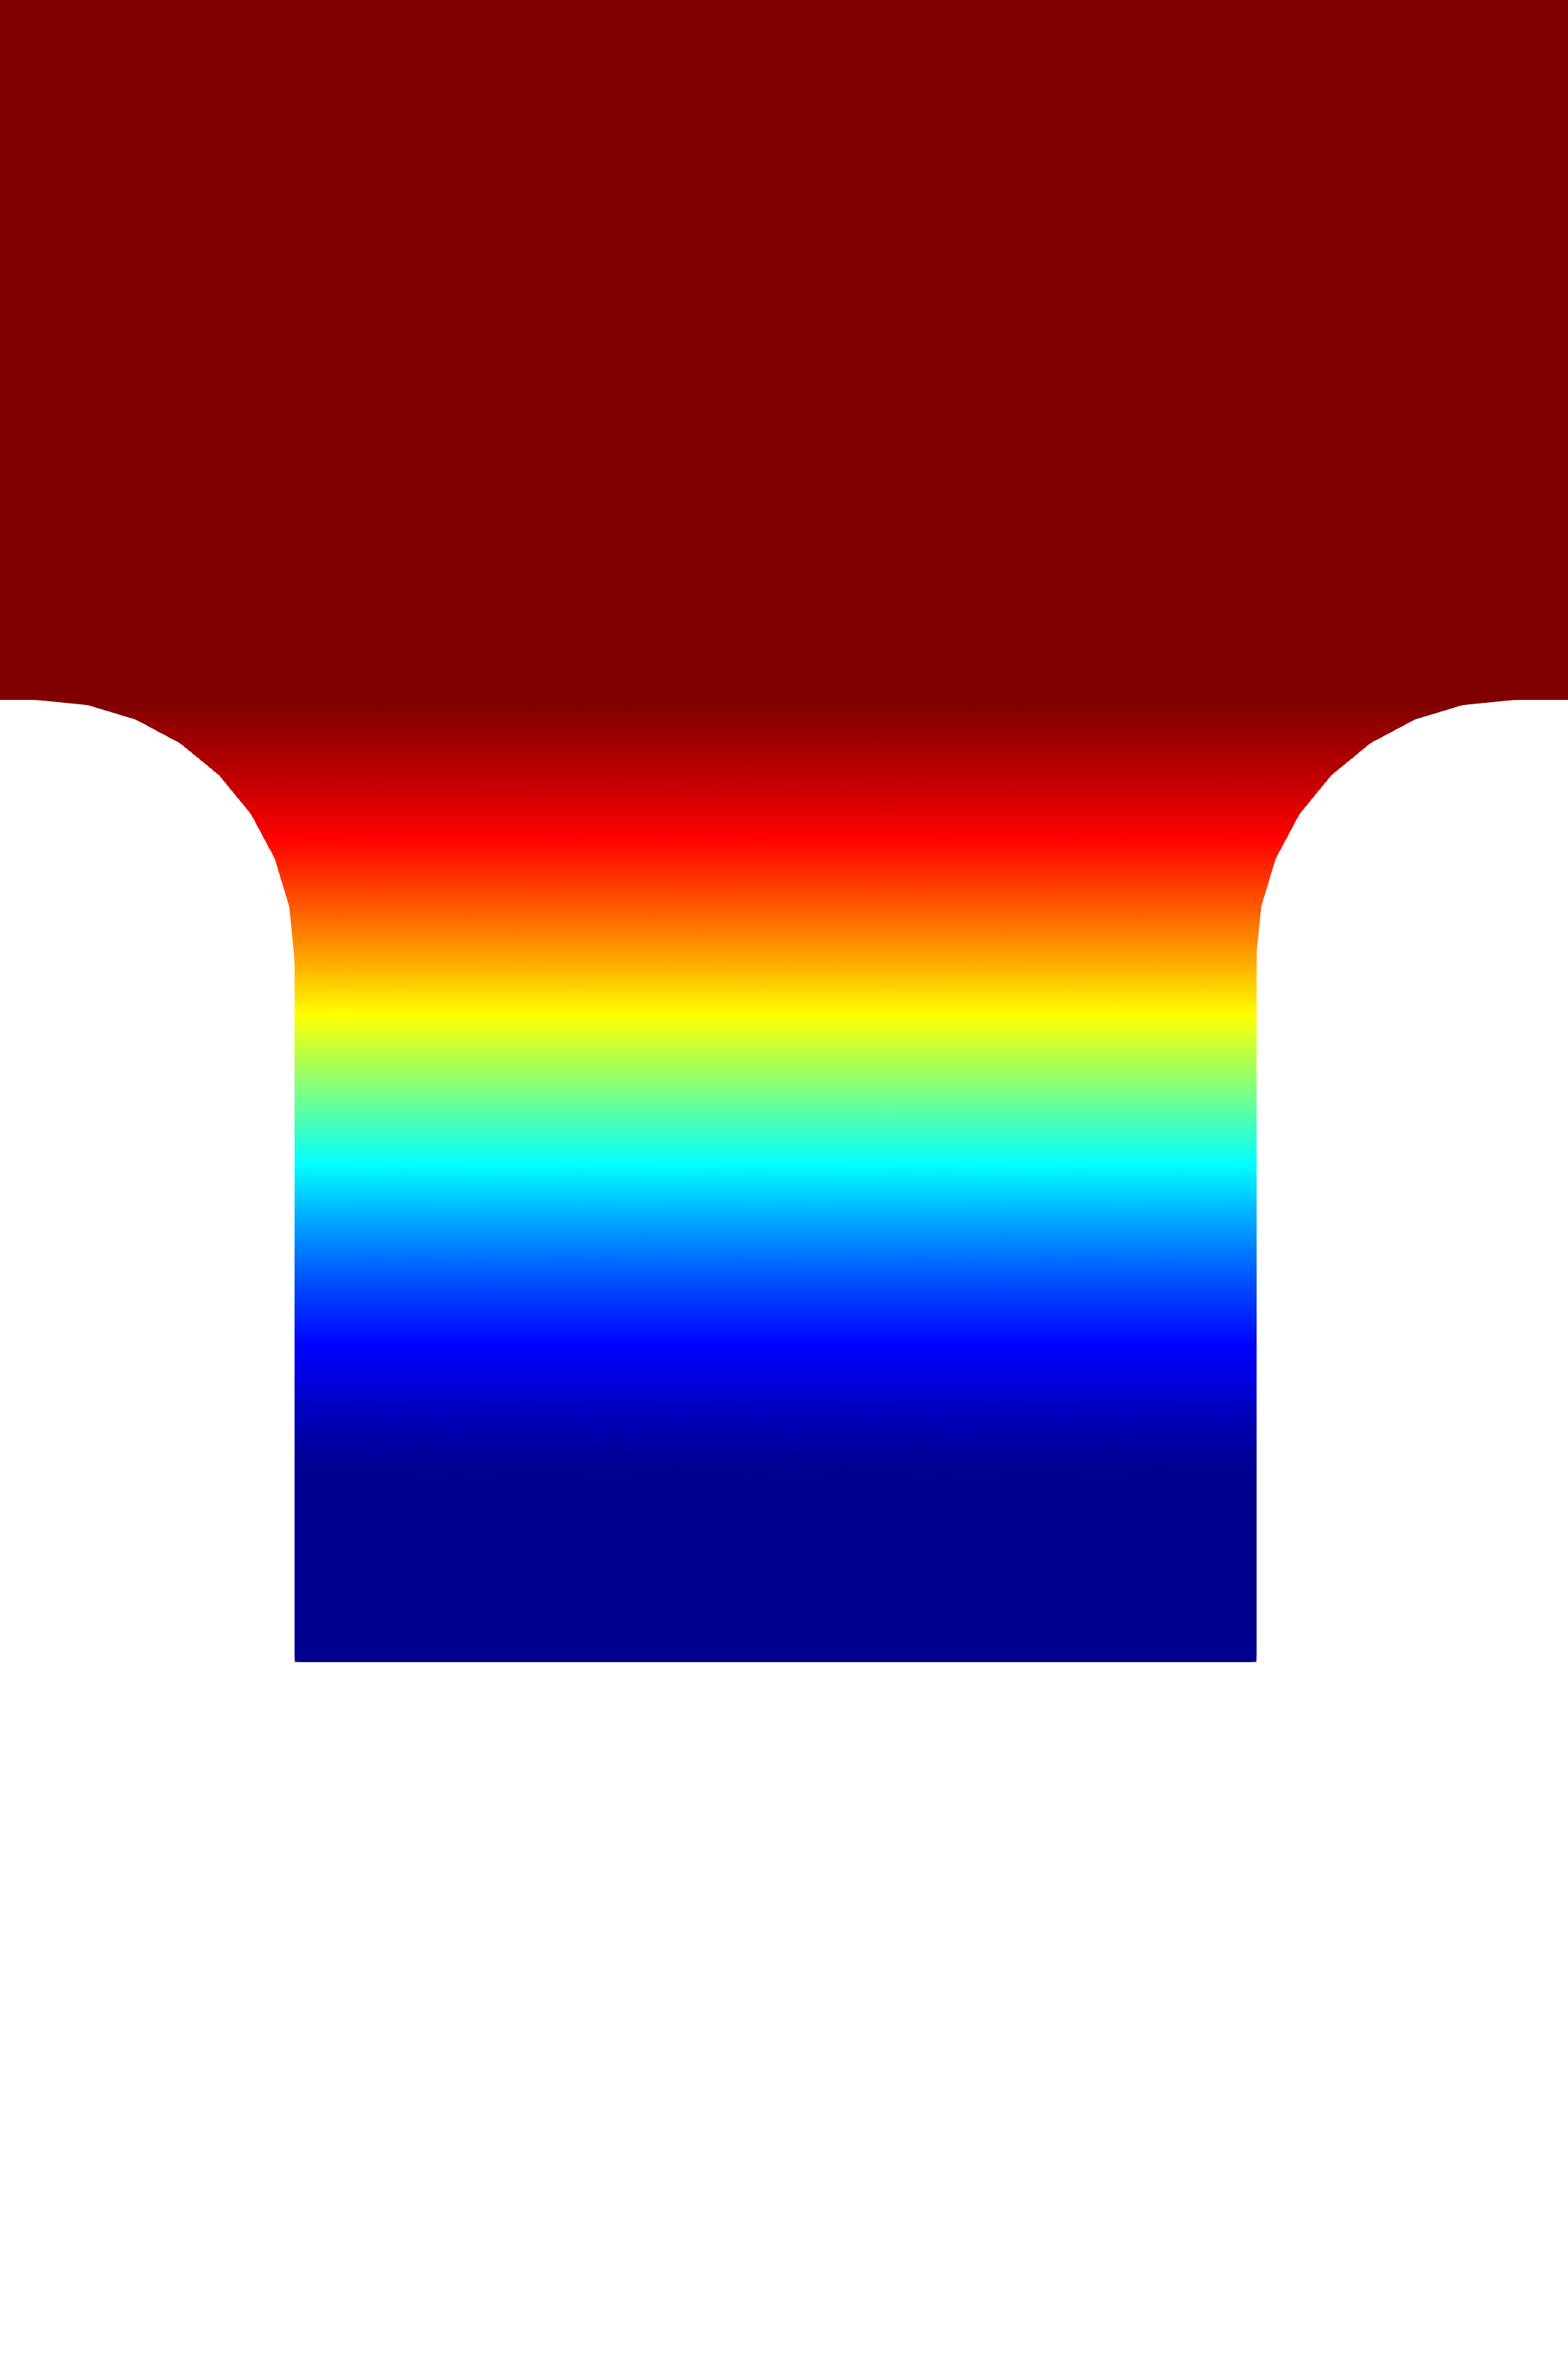
\includegraphics[width=82.5pt,height=123.83pt]{diagrams/results-modelling/velocity-transport/meshandsoln_cg_permeability_placenta_nsb_permeability-linear_vein.png}};
%Shape: Polygon [id:ds7395586031334473] 
\draw  [fill={rgb, 255:red, 155; green, 155; blue, 155 }  ,fill opacity=0.2 ] (421.25,250.25) -- (317,245.5) -- (317,120) -- (421.25,23) -- cycle ;
%Shape: Rectangle [id:dp1357774358505115] 
\draw   (240.75,120) -- (317,120) -- (317,245.5) -- (240.75,245.5) -- cycle ;
%Shape: Rectangle [id:dp02134536760375405] 
\draw  [color={rgb, 255:red, 144; green, 19; blue, 254 }  ,draw opacity=1 ][fill={rgb, 255:red, 255; green, 255; blue, 255 }  ,fill opacity=1 ][line width=2.25] [blur shadow={shadow xshift=0pt,shadow yshift=0pt, shadow blur radius=1.5pt, shadow blur steps=4 ,shadow opacity=100}] (421.25,23) -- (576.5,23) -- (576.5,250.5) -- (421.25,250.5) -- cycle ;
%Image [id:dp27582567302078576] 
\draw (497.74,131.58) node  {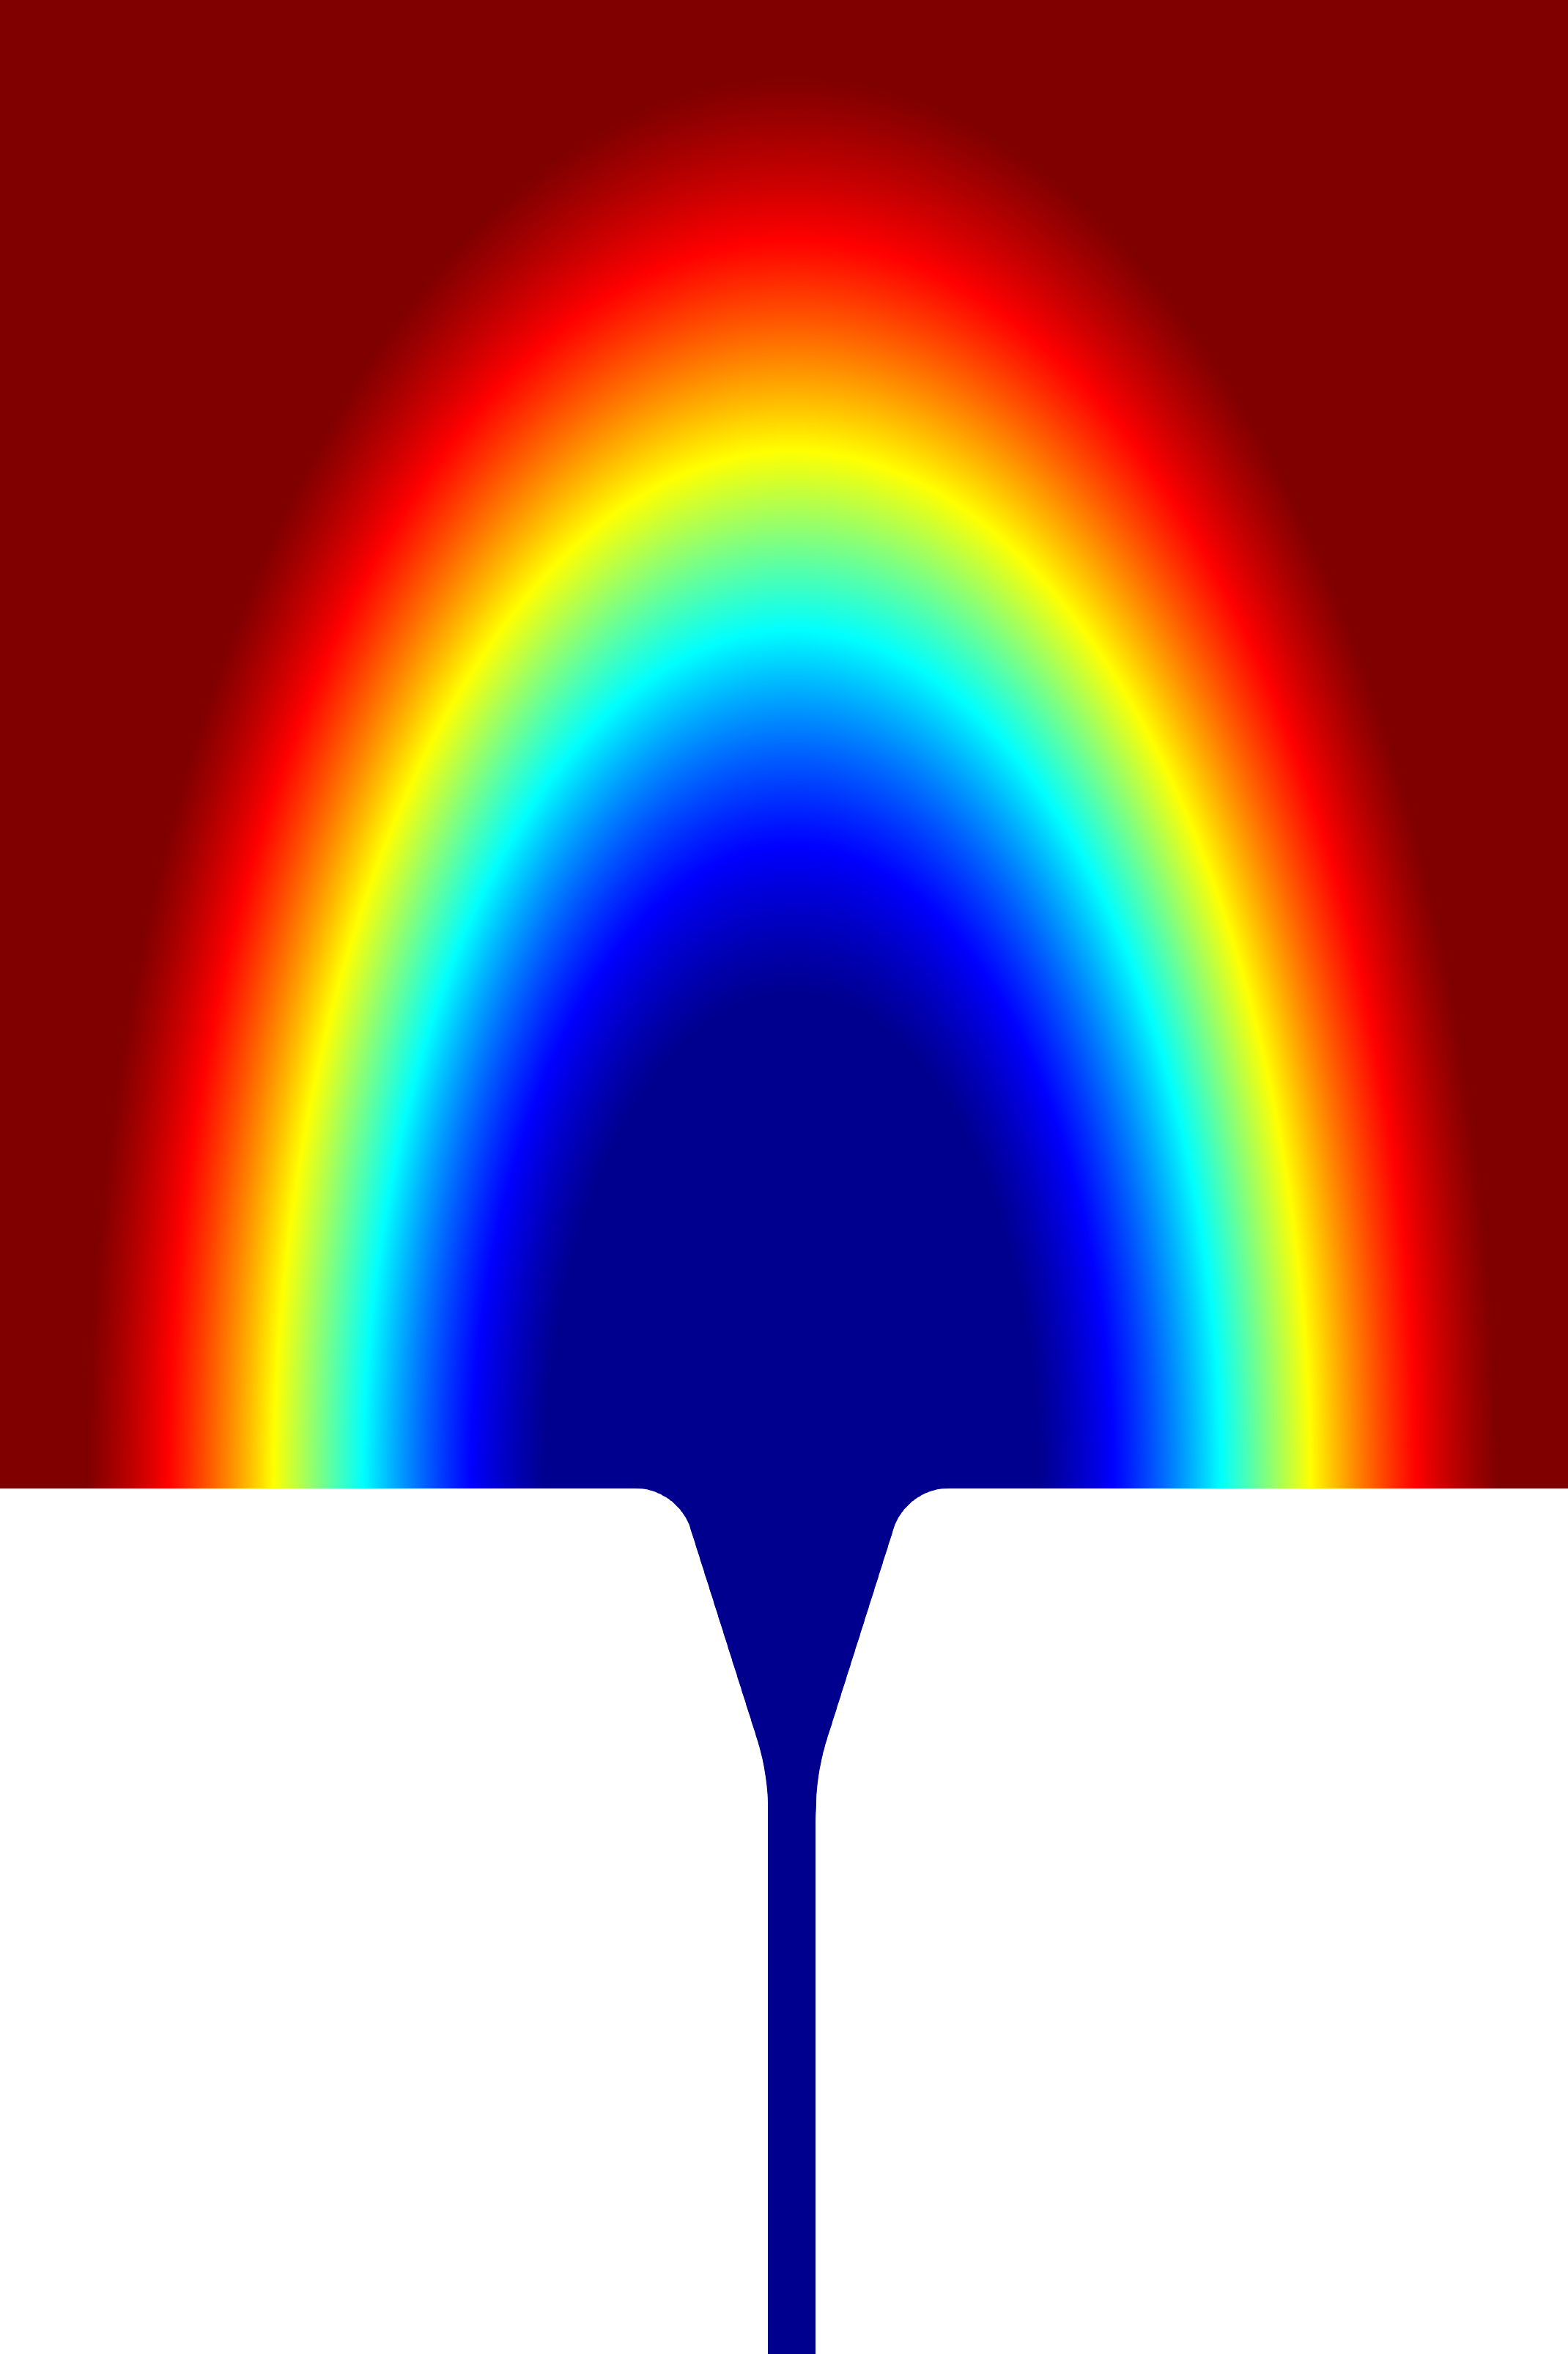
\includegraphics[width=101.85pt,height=152.88pt]{diagrams/results-modelling/velocity-transport/meshandsoln_cg_permeability_placenta_nsb_permeability-linear_cavity.png}};
%Shape: Polygon [id:ds4671748834121485] 
\draw  [fill={rgb, 255:red, 155; green, 155; blue, 155 }  ,fill opacity=0.2 ] (217.75,202.5) -- (160,218) -- (160,74.5) -- (217.75,186.5) -- cycle ;
%Shape: Rectangle [id:dp28400651386966036] 
\draw   (217.75,186.5) -- (231,186.5) -- (231,202.5) -- (217.75,202.5) -- cycle ;




\end{tikzpicture}
